% Created by tikzDevice version 0.12.6 on 2024-07-27 08:39:08
% !TEX encoding = UTF-8 Unicode
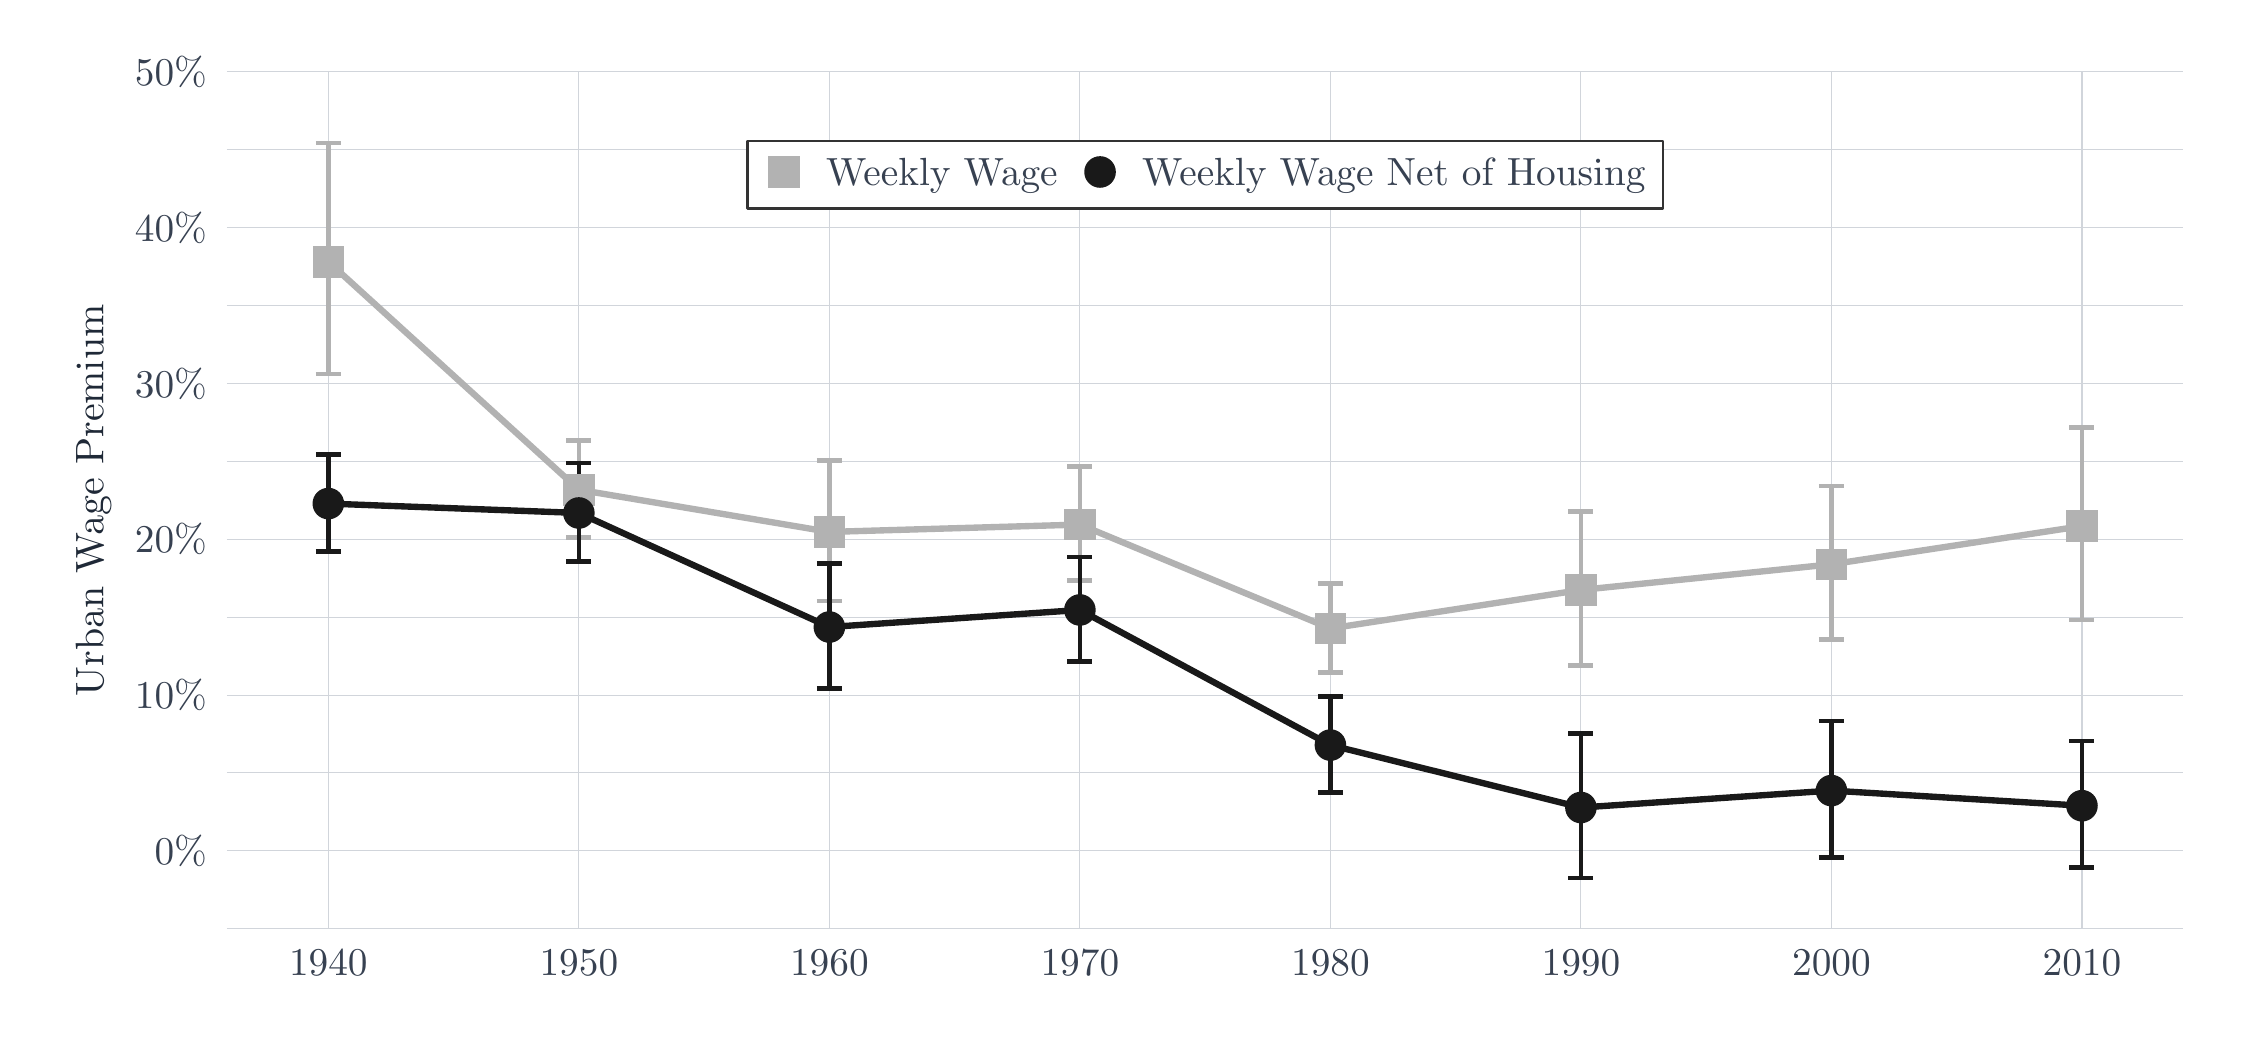
\begin{tikzpicture}[x=1pt,y=1pt]
\definecolor{fillColor}{RGB}{255,255,255}
\path[use as bounding box,fill=fillColor] (0,0) rectangle (794.97,361.35);
\begin{scope}
\path[clip] (  0.00,  0.00) rectangle (794.97,361.35);
\definecolor{drawColor}{RGB}{255,255,255}

\path[draw=drawColor,line width= 0.8pt,line join=round,line cap=round,fill=fillColor] (  0.00,  0.00) rectangle (794.97,361.35);
\end{scope}
\begin{scope}
\path[clip] ( 71.98, 35.76) rectangle (778.97,345.35);
\definecolor{drawColor}{RGB}{255,255,255}
\definecolor{fillColor}{RGB}{255,255,255}

\path[draw=drawColor,line width= 0.8pt,line join=round,line cap=round,fill=fillColor] ( 71.98, 35.76) rectangle (778.97,345.35);
\definecolor{drawColor}{RGB}{209,213,219}

\path[draw=drawColor,line width= 0.4pt,line join=round] ( 71.98, 35.76) --
	(778.97, 35.76);

\path[draw=drawColor,line width= 0.4pt,line join=round] ( 71.98, 92.05) --
	(778.97, 92.05);

\path[draw=drawColor,line width= 0.4pt,line join=round] ( 71.98,148.34) --
	(778.97,148.34);

\path[draw=drawColor,line width= 0.4pt,line join=round] ( 71.98,204.63) --
	(778.97,204.63);

\path[draw=drawColor,line width= 0.4pt,line join=round] ( 71.98,260.92) --
	(778.97,260.92);

\path[draw=drawColor,line width= 0.4pt,line join=round] ( 71.98,317.21) --
	(778.97,317.21);

\path[draw=drawColor,line width= 0.4pt,line join=round] ( 71.98, 63.90) --
	(778.97, 63.90);

\path[draw=drawColor,line width= 0.4pt,line join=round] ( 71.98,120.19) --
	(778.97,120.19);

\path[draw=drawColor,line width= 0.4pt,line join=round] ( 71.98,176.48) --
	(778.97,176.48);

\path[draw=drawColor,line width= 0.4pt,line join=round] ( 71.98,232.77) --
	(778.97,232.77);

\path[draw=drawColor,line width= 0.4pt,line join=round] ( 71.98,289.06) --
	(778.97,289.06);

\path[draw=drawColor,line width= 0.4pt,line join=round] ( 71.98,345.35) --
	(778.97,345.35);

\path[draw=drawColor,line width= 0.4pt,line join=round] (108.64, 35.76) --
	(108.64,345.35);

\path[draw=drawColor,line width= 0.4pt,line join=round] (199.17, 35.76) --
	(199.17,345.35);

\path[draw=drawColor,line width= 0.4pt,line join=round] (289.69, 35.76) --
	(289.69,345.35);

\path[draw=drawColor,line width= 0.4pt,line join=round] (380.21, 35.76) --
	(380.21,345.35);

\path[draw=drawColor,line width= 0.4pt,line join=round] (470.74, 35.76) --
	(470.74,345.35);

\path[draw=drawColor,line width= 0.4pt,line join=round] (561.26, 35.76) --
	(561.26,345.35);

\path[draw=drawColor,line width= 0.4pt,line join=round] (651.78, 35.76) --
	(651.78,345.35);

\path[draw=drawColor,line width= 0.4pt,line join=round] (742.31, 35.76) --
	(742.31,345.35);
\definecolor{drawColor}{gray}{0.70}

\path[draw=drawColor,line width= 2.3pt,line join=round] (108.64,276.78) --
	(199.17,194.38) --
	(289.69,179.14) --
	(380.21,181.79) --
	(470.74,144.26) --
	(561.26,158.17) --
	(651.78,167.43) --
	(742.31,181.24);
\definecolor{drawColor}{gray}{0.10}

\path[draw=drawColor,line width= 2.3pt,line join=round] (108.64,189.38) --
	(199.17,185.98) --
	(289.69,144.77) --
	(380.21,150.94) --
	(470.74,102.11) --
	(561.26, 79.55) --
	(651.78, 85.67) --
	(742.31, 80.20);
\definecolor{drawColor}{gray}{0.70}

\path[draw=drawColor,line width= 1.7pt,line join=round] (104.12,319.64) --
	(113.17,319.64);

\path[draw=drawColor,line width= 1.7pt,line join=round] (108.64,319.64) --
	(108.64,236.16);

\path[draw=drawColor,line width= 1.7pt,line join=round] (104.12,236.16) --
	(113.17,236.16);
\definecolor{drawColor}{gray}{0.10}

\path[draw=drawColor,line width= 1.7pt,line join=round] (104.12,207.03) --
	(113.17,207.03);

\path[draw=drawColor,line width= 1.7pt,line join=round] (108.64,207.03) --
	(108.64,172.17);

\path[draw=drawColor,line width= 1.7pt,line join=round] (104.12,172.17) --
	(113.17,172.17);
\definecolor{drawColor}{gray}{0.70}

\path[draw=drawColor,line width= 1.7pt,line join=round] (194.64,212.07) --
	(203.69,212.07);

\path[draw=drawColor,line width= 1.7pt,line join=round] (199.17,212.07) --
	(199.17,177.12);

\path[draw=drawColor,line width= 1.7pt,line join=round] (194.64,177.12) --
	(203.69,177.12);
\definecolor{drawColor}{gray}{0.10}

\path[draw=drawColor,line width= 1.7pt,line join=round] (194.64,204.01) --
	(203.69,204.01);

\path[draw=drawColor,line width= 1.7pt,line join=round] (199.17,204.01) --
	(199.17,168.42);

\path[draw=drawColor,line width= 1.7pt,line join=round] (194.64,168.42) --
	(203.69,168.42);
\definecolor{drawColor}{gray}{0.70}

\path[draw=drawColor,line width= 1.7pt,line join=round] (285.16,205.07) --
	(294.22,205.07);

\path[draw=drawColor,line width= 1.7pt,line join=round] (289.69,205.07) --
	(289.69,154.17);

\path[draw=drawColor,line width= 1.7pt,line join=round] (285.16,154.17) --
	(294.22,154.17);
\definecolor{drawColor}{gray}{0.10}

\path[draw=drawColor,line width= 1.7pt,line join=round] (285.16,167.70) --
	(294.22,167.70);

\path[draw=drawColor,line width= 1.7pt,line join=round] (289.69,167.70) --
	(289.69,122.63);

\path[draw=drawColor,line width= 1.7pt,line join=round] (285.16,122.63) --
	(294.22,122.63);
\definecolor{drawColor}{gray}{0.70}

\path[draw=drawColor,line width= 1.7pt,line join=round] (375.69,202.68) --
	(384.74,202.68);

\path[draw=drawColor,line width= 1.7pt,line join=round] (380.21,202.68) --
	(380.21,161.53);

\path[draw=drawColor,line width= 1.7pt,line join=round] (375.69,161.53) --
	(384.74,161.53);
\definecolor{drawColor}{gray}{0.10}

\path[draw=drawColor,line width= 1.7pt,line join=round] (375.69,170.05) --
	(384.74,170.05);

\path[draw=drawColor,line width= 1.7pt,line join=round] (380.21,170.05) --
	(380.21,132.38);

\path[draw=drawColor,line width= 1.7pt,line join=round] (375.69,132.38) --
	(384.74,132.38);
\definecolor{drawColor}{gray}{0.70}

\path[draw=drawColor,line width= 1.7pt,line join=round] (466.21,160.48) --
	(475.26,160.48);

\path[draw=drawColor,line width= 1.7pt,line join=round] (470.74,160.48) --
	(470.74,128.44);

\path[draw=drawColor,line width= 1.7pt,line join=round] (466.21,128.44) --
	(475.26,128.44);
\definecolor{drawColor}{gray}{0.10}

\path[draw=drawColor,line width= 1.7pt,line join=round] (466.21,119.79) --
	(475.26,119.79);

\path[draw=drawColor,line width= 1.7pt,line join=round] (470.74,119.79) --
	(470.74, 84.94);

\path[draw=drawColor,line width= 1.7pt,line join=round] (466.21, 84.94) --
	(475.26, 84.94);
\definecolor{drawColor}{gray}{0.70}

\path[draw=drawColor,line width= 1.7pt,line join=round] (556.73,186.62) --
	(565.79,186.62);

\path[draw=drawColor,line width= 1.7pt,line join=round] (561.26,186.62) --
	(561.26,130.89);

\path[draw=drawColor,line width= 1.7pt,line join=round] (556.73,130.89) --
	(565.79,130.89);
\definecolor{drawColor}{gray}{0.10}

\path[draw=drawColor,line width= 1.7pt,line join=round] (556.73,106.19) --
	(565.79,106.19);

\path[draw=drawColor,line width= 1.7pt,line join=round] (561.26,106.19) --
	(561.26, 54.09);

\path[draw=drawColor,line width= 1.7pt,line join=round] (556.73, 54.09) --
	(565.79, 54.09);
\definecolor{drawColor}{gray}{0.70}

\path[draw=drawColor,line width= 1.7pt,line join=round] (647.26,195.77) --
	(656.31,195.77);

\path[draw=drawColor,line width= 1.7pt,line join=round] (651.78,195.77) --
	(651.78,140.25);

\path[draw=drawColor,line width= 1.7pt,line join=round] (647.26,140.25) --
	(656.31,140.25);
\definecolor{drawColor}{gray}{0.10}

\path[draw=drawColor,line width= 1.7pt,line join=round] (647.26,110.79) --
	(656.31,110.79);

\path[draw=drawColor,line width= 1.7pt,line join=round] (651.78,110.79) --
	(651.78, 61.58);

\path[draw=drawColor,line width= 1.7pt,line join=round] (647.26, 61.58) --
	(656.31, 61.58);
\definecolor{drawColor}{gray}{0.70}

\path[draw=drawColor,line width= 1.7pt,line join=round] (737.78,216.95) --
	(746.83,216.95);

\path[draw=drawColor,line width= 1.7pt,line join=round] (742.31,216.95) --
	(742.31,147.31);

\path[draw=drawColor,line width= 1.7pt,line join=round] (737.78,147.31) --
	(746.83,147.31);
\definecolor{drawColor}{gray}{0.10}

\path[draw=drawColor,line width= 1.7pt,line join=round] (737.78,103.54) --
	(746.83,103.54);

\path[draw=drawColor,line width= 1.7pt,line join=round] (742.31,103.54) --
	(742.31, 57.78);

\path[draw=drawColor,line width= 1.7pt,line join=round] (737.78, 57.78) --
	(746.83, 57.78);
\definecolor{fillColor}{gray}{0.70}

\path[fill=fillColor] (102.93,271.07) --
	(114.35,271.07) --
	(114.35,282.49) --
	(102.93,282.49) --
	cycle;
\definecolor{fillColor}{gray}{0.10}

\path[fill=fillColor] (108.64,189.38) circle (  5.71);
\definecolor{fillColor}{gray}{0.70}

\path[fill=fillColor] (193.46,188.67) --
	(204.88,188.67) --
	(204.88,200.09) --
	(193.46,200.09) --
	cycle;
\definecolor{fillColor}{gray}{0.10}

\path[fill=fillColor] (199.17,185.98) circle (  5.71);
\definecolor{fillColor}{gray}{0.70}

\path[fill=fillColor] (283.98,173.43) --
	(295.40,173.43) --
	(295.40,184.85) --
	(283.98,184.85) --
	cycle;
\definecolor{fillColor}{gray}{0.10}

\path[fill=fillColor] (289.69,144.77) circle (  5.71);
\definecolor{fillColor}{gray}{0.70}

\path[fill=fillColor] (374.50,176.08) --
	(385.92,176.08) --
	(385.92,187.50) --
	(374.50,187.50) --
	cycle;
\definecolor{fillColor}{gray}{0.10}

\path[fill=fillColor] (380.21,150.94) circle (  5.71);
\definecolor{fillColor}{gray}{0.70}

\path[fill=fillColor] (465.03,138.55) --
	(476.45,138.55) --
	(476.45,149.97) --
	(465.03,149.97) --
	cycle;
\definecolor{fillColor}{gray}{0.10}

\path[fill=fillColor] (470.74,102.11) circle (  5.71);
\definecolor{fillColor}{gray}{0.70}

\path[fill=fillColor] (555.55,152.46) --
	(566.97,152.46) --
	(566.97,163.88) --
	(555.55,163.88) --
	cycle;
\definecolor{fillColor}{gray}{0.10}

\path[fill=fillColor] (561.26, 79.55) circle (  5.71);
\definecolor{fillColor}{gray}{0.70}

\path[fill=fillColor] (646.07,161.72) --
	(657.49,161.72) --
	(657.49,173.14) --
	(646.07,173.14) --
	cycle;
\definecolor{fillColor}{gray}{0.10}

\path[fill=fillColor] (651.78, 85.67) circle (  5.71);
\definecolor{fillColor}{gray}{0.70}

\path[fill=fillColor] (736.60,175.53) --
	(748.02,175.53) --
	(748.02,186.95) --
	(736.60,186.95) --
	cycle;
\definecolor{fillColor}{gray}{0.10}

\path[fill=fillColor] (742.31, 80.20) circle (  5.71);
\end{scope}
\begin{scope}
\path[clip] (  0.00,  0.00) rectangle (794.97,361.35);
\definecolor{drawColor}{RGB}{55,65,81}

\node[text=drawColor,anchor=base east,inner sep=0pt, outer sep=0pt, scale=  1.42] at ( 64.78, 59.01) {0\%};

\node[text=drawColor,anchor=base east,inner sep=0pt, outer sep=0pt, scale=  1.42] at ( 64.78,115.30) {10\%};

\node[text=drawColor,anchor=base east,inner sep=0pt, outer sep=0pt, scale=  1.42] at ( 64.78,171.58) {20\%};

\node[text=drawColor,anchor=base east,inner sep=0pt, outer sep=0pt, scale=  1.42] at ( 64.78,227.87) {30\%};

\node[text=drawColor,anchor=base east,inner sep=0pt, outer sep=0pt, scale=  1.42] at ( 64.78,284.16) {40\%};

\node[text=drawColor,anchor=base east,inner sep=0pt, outer sep=0pt, scale=  1.42] at ( 64.78,340.45) {50\%};
\end{scope}
\begin{scope}
\path[clip] (  0.00,  0.00) rectangle (794.97,361.35);
\definecolor{drawColor}{RGB}{55,65,81}

\node[text=drawColor,anchor=base,inner sep=0pt, outer sep=0pt, scale=  1.42] at (108.64, 18.76) {1940};

\node[text=drawColor,anchor=base,inner sep=0pt, outer sep=0pt, scale=  1.42] at (199.17, 18.76) {1950};

\node[text=drawColor,anchor=base,inner sep=0pt, outer sep=0pt, scale=  1.42] at (289.69, 18.76) {1960};

\node[text=drawColor,anchor=base,inner sep=0pt, outer sep=0pt, scale=  1.42] at (380.21, 18.76) {1970};

\node[text=drawColor,anchor=base,inner sep=0pt, outer sep=0pt, scale=  1.42] at (470.74, 18.76) {1980};

\node[text=drawColor,anchor=base,inner sep=0pt, outer sep=0pt, scale=  1.42] at (561.26, 18.76) {1990};

\node[text=drawColor,anchor=base,inner sep=0pt, outer sep=0pt, scale=  1.42] at (651.78, 18.76) {2000};

\node[text=drawColor,anchor=base,inner sep=0pt, outer sep=0pt, scale=  1.42] at (742.31, 18.76) {2010};
\end{scope}
\begin{scope}
\path[clip] (  0.00,  0.00) rectangle (794.97,361.35);
\definecolor{drawColor}{RGB}{31,41,55}

\node[text=drawColor,rotate= 90.00,anchor=base,inner sep=0pt, outer sep=0pt, scale=  1.44] at ( 27.32,190.55) {Urban Wage Premium};
\end{scope}
\begin{scope}
\path[clip] (  0.00,  0.00) rectangle (794.97,361.35);
\definecolor{drawColor}{gray}{0.20}
\definecolor{fillColor}{RGB}{255,255,255}

\path[draw=drawColor,line width= 0.8pt,line join=round,line cap=round,fill=fillColor] (260.10,295.97) rectangle (590.85,320.43);
\end{scope}
\begin{scope}
\path[clip] (  0.00,  0.00) rectangle (794.97,361.35);
\definecolor{drawColor}{RGB}{255,255,255}
\definecolor{fillColor}{RGB}{255,255,255}

\path[draw=drawColor,line width= 0.8pt,line join=round,line cap=round,fill=fillColor] (266.10,301.97) rectangle (280.55,316.43);
\end{scope}
\begin{scope}
\path[clip] (  0.00,  0.00) rectangle (794.97,361.35);
\definecolor{fillColor}{gray}{0.70}

\path[fill=fillColor] (267.61,303.49) --
	(279.03,303.49) --
	(279.03,314.91) --
	(267.61,314.91) --
	cycle;
\end{scope}
\begin{scope}
\path[clip] (  0.00,  0.00) rectangle (794.97,361.35);
\definecolor{drawColor}{RGB}{255,255,255}
\definecolor{fillColor}{RGB}{255,255,255}

\path[draw=drawColor,line width= 0.8pt,line join=round,line cap=round,fill=fillColor] (380.27,301.97) rectangle (394.72,316.43);
\end{scope}
\begin{scope}
\path[clip] (  0.00,  0.00) rectangle (794.97,361.35);
\definecolor{fillColor}{gray}{0.10}

\path[fill=fillColor] (387.50,309.20) circle (  5.71);
\end{scope}
\begin{scope}
\path[clip] (  0.00,  0.00) rectangle (794.97,361.35);
\definecolor{drawColor}{RGB}{55,65,81}

\node[text=drawColor,anchor=base west,inner sep=0pt, outer sep=0pt, scale=  1.42] at (288.55,304.30) {Weekly Wage};
\end{scope}
\begin{scope}
\path[clip] (  0.00,  0.00) rectangle (794.97,361.35);
\definecolor{drawColor}{RGB}{55,65,81}

\node[text=drawColor,anchor=base west,inner sep=0pt, outer sep=0pt, scale=  1.42] at (402.72,304.30) {Weekly Wage Net of Housing};
\end{scope}
\end{tikzpicture}
